\chapter{Integrated System}
\label{ch:integrated}

The three previous chapters each solved one perception sub-task in isolation, on
its own data and against its own metric: locating the ball in every frame
(Chapter~\ref{ch:ball}), registering the playing surface
(Chapter~\ref{ch:court}), and timing the bounces along the resulting trajectory
(Chapter~\ref{ch:bounce}). This chapter combines the three selected models into a
single system that ingests a raw clip and emits one annotated video, and it adds
the step that motivates the whole system: projecting each bounce onto the court
through the estimated homography and deciding, by polygon containment, whether the
ball landed in or out. That composition is the subject of the fourth research
question (RQ4) of Section~\ref{sec:intro-objectives}: whether the best models of
the three sub-tasks can be wired into one end-to-end pipeline that produces tracked
ball, court geometry, bounce events, and a per-bounce line call. The line call is
presented here as a qualitative geometric capability, for the reason developed in
Section~\ref{sec:int-inout} and already flagged in Section~\ref{sec:bounce-analysis}:
the datasets carry no ground-truth in-or-out labels against which it could be
scored.

\section{Architecture}
\label{sec:int-arch}

The integrated system is an orchestration layer over the three component
models. A single entry point reads a video, runs the three models in turn, performs the line-call
geometry, and writes an annotated MP4 together with a summary record.
Figure~\ref{fig:int-pipeline} shows the data flow. The three perception modules are
not retrained or modified here; each is loaded from the checkpoint selected in its
own chapter and wrapped behind a uniform inference call, so that the integration
concerns only how their outputs are combined.

\begin{figure}[t]
  \centering
  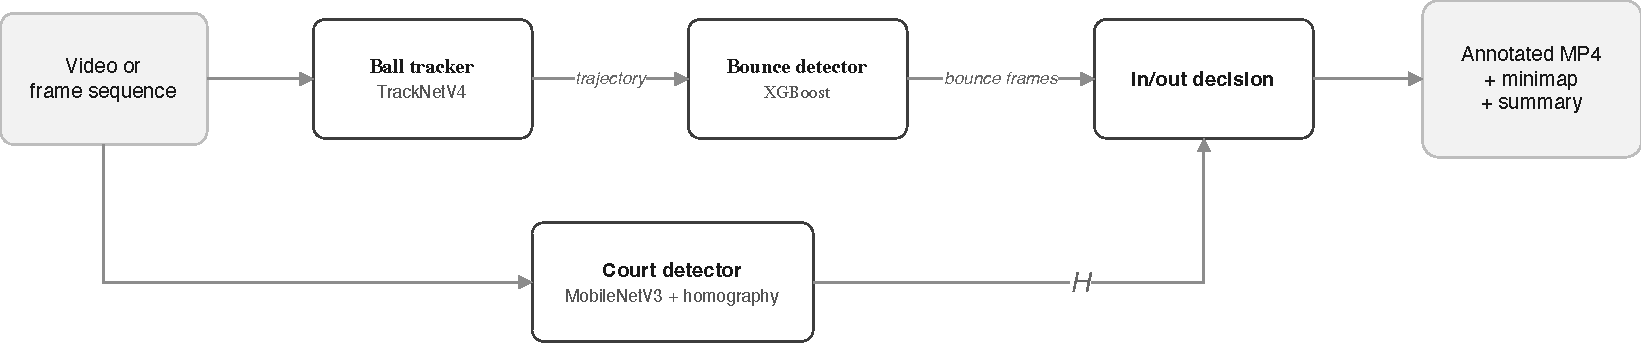
\includegraphics[width=\linewidth]{img/integrated_pipeline.pdf}
  \caption{Data flow of the integrated pipeline. The ball tracker and the court
    detector both consume the input frames; the ball tracker yields a per-frame
    trajectory and the court detector yields a frame-pixel-to-court-metre
    homography $H$. The bounce detector marks bounce frames along the trajectory,
    and the in/out stage projects the ball's position at each bounce through $H$ and
    tests court-polygon containment. All outputs are composited into one annotated
    video with a top-down court minimap and a summary record.}
  \label{fig:int-pipeline}
\end{figure}

The pipeline runs the models in a fixed order, each stage consuming the previous
output. The ball tracker is run first over every frame, producing the trajectory in
its native $640 \times 368$ working resolution, which is then scaled to the
original frame size. The court detector is run on the opening frames
until one yields a valid homography: its keypoints, predicted in a $640 \times 360$
space, are scaled to the original frame size and passed to the RANSAC homography fit
of Section~\ref{sec:court-homography}, and the first frame that produces a usable
$H$ fixes the court geometry for the clip. The bounce detector then runs on the scaled trajectory, and
finally the line-call stage of Section~\ref{sec:int-inout} consumes the trajectory,
the homography, and the detected bounce frames together. The orchestrator returns a
summary record reporting the number of bounces, the in and out counts, the line-call
quality flag, and the measured throughput of the ball and court stages.

\section{In/Out Line Call}
\label{sec:int-inout}

The line call is the step that turns three streams of perception output into the
decision the system is named for. It rests on the homography $H$ of
Section~\ref{sec:court-homography}, which maps a point in frame pixels to its
position on the court in metres. For each detected bounce at which the ball is
visible, the pipeline takes the ball's frame-pixel position at that frame and
projects it through $H$ to a court-metre coordinate, then tests whether that point
lies inside the court polygon. The polygon is the singles or the doubles court, a
choice exposed to the user, expressed as four corner coordinates in the same
court-metre frame as $H$. A bounce that projects inside the polygon is labelled
IN, one outside is labelled OUT.


The honesty of this output must be stated as carefully as its mechanism, and the
qualification is the same one raised in Section~\ref{sec:bounce-analysis}. The line
call is a geometric demonstration, not a validated measurement. Neither dataset of
this thesis carries a ground-truth in-or-out annotation, so there is no label against
which a projected call could be scored, and no accuracy, precision, or error rate for
the line call is reported anywhere in this work.

\section{End-to-End Demonstration}
\label{sec:int-demo}

The complete pipeline was run on a held-out clip from match game10, the same test
match as the ball tracker's final evaluation (Section~\ref{sec:ball-final}), to
exercise every stage on data no component had trained on.
Figure~\ref{fig:int-demo} shows a representative annotated frame. The ball trail, the
IN banner, the expanding ring at the detected bounce, and the court minimap
with its projected trajectory and bounce markers are all visible together, which is
the qualitative evidence that the composition of Section~\ref{sec:int-arch} works
end to end: the trajectory from TrackNetV4, the homography from MobileNetV3, and the
bounce timing from XGBoost combine into a single coherent annotation, and the
homography projection places the bounces sensibly within the court on the minimap.

\begin{figure}[t]
  \centering
  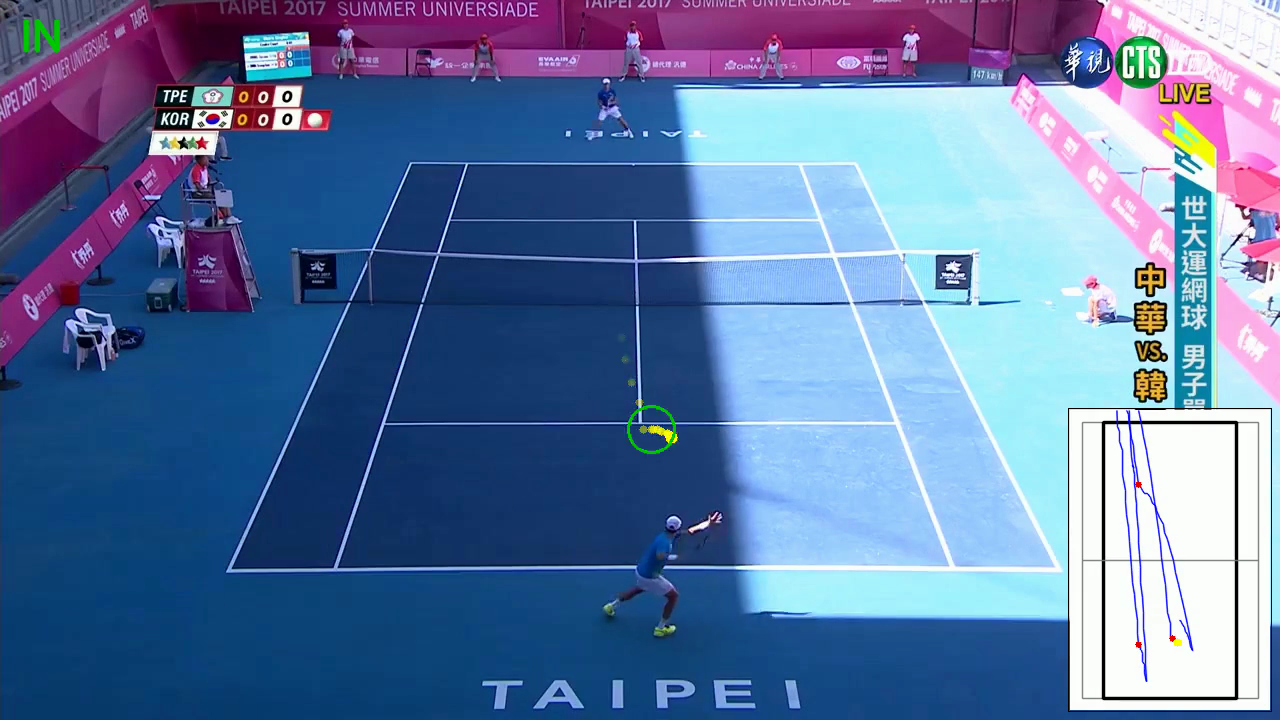
\includegraphics[width=\linewidth]{img/integrated_demo_frame.png}
  \caption{A representative frame from the end-to-end demonstration on a game10 test
    clip. The ball is tracked with a fading trail (yellow); a detected bounce is
    marked by an expanding ring on the court and announced by the banner at the top
    left, here IN (green). The court minimap composited into the bottom-right
    corner shows the singles and doubles court lines, the ball trajectory projected
    into court-metre space (blue), the bounce positions accumulated so far (red), and
    the current ball position (yellow). The line call is a qualitative geometric
    output, not a validated measurement (Section~\ref{sec:int-inout}).}
  \label{fig:int-demo}
\end{figure}


This demonstration answers RQ4. The three models selected on their own sub-tasks do
compose into a single program that takes a raw clip and emits a tracked ball, a
registered court, timed bounces, and a per-bounce in-or-out call. The line call, the application that motivates the
system, is realised as a working geometric capability, with the clear and repeated
caveat that it is qualitative: a demonstration of the pipeline's reach, awaiting the
labelled data and uncertainty modelling that quantitative officiating-grade
validation would require.
